\documentclass[11pt,oneside,a4paper]{article}
\usepackage{graphicx}
\usepackage{hyperref}

\title{Hello}


\title{Integrating Knowledge Graphs into the Debian Ecosystem}
\author{Alexander Belikov \\ \href{mailto:alexander@growgraph.dev}{alexander@growgraph.dev}}
\date{June 2025}

\begin{document}

    \maketitle

    \begin{abstract}
        In an era where software systems are increasingly complex and interconnected, understanding and managing the relationships between packages, maintainers, dependencies, and vulnerabilities is paramount.
        We the innovative integration of knowledge graphs into the Debian ecosystem, offering a structured and semantic approach to package management and analysis.
        We delve into how knowledge graphs can unify diverse data sources — such as package metadata, security advisories, and reproducibility reports — into an interconnected model that enhances visibility and enables insights and optimization suggestions at levels unattainable for non-graph engines.
    \end{abstract}


    \section{Introduction}

    Knowledge Graphs, known as semantic web previously have become ubiquitous.
    While their applications to large-scale project management is fairly recent, they were used to normalize web resources with <schema.org> \cite{Iliadis2023-cm} etc [give more examples]



    Debian is a leading linux distribution, serving as foundation for a large share of modern infrastructure.
    At the same time it is a complex ecosystem, interconnected at many levels.

    It is critical to optimize debian workflow not only from the point of view of saving time, but also direct towards updates in most critical areas, reduce uncertainty about future updates, enhance robustness.
    Connect external data sources to learn (some bugs are not reported) which way to direct it.


    Importance of implicit interactions between code and people (often unique expertise).


    \section{Related Work}


    \section{Schema}

    \begin{figure}[h]
        \centering
        \begin{tabular}{cc}
            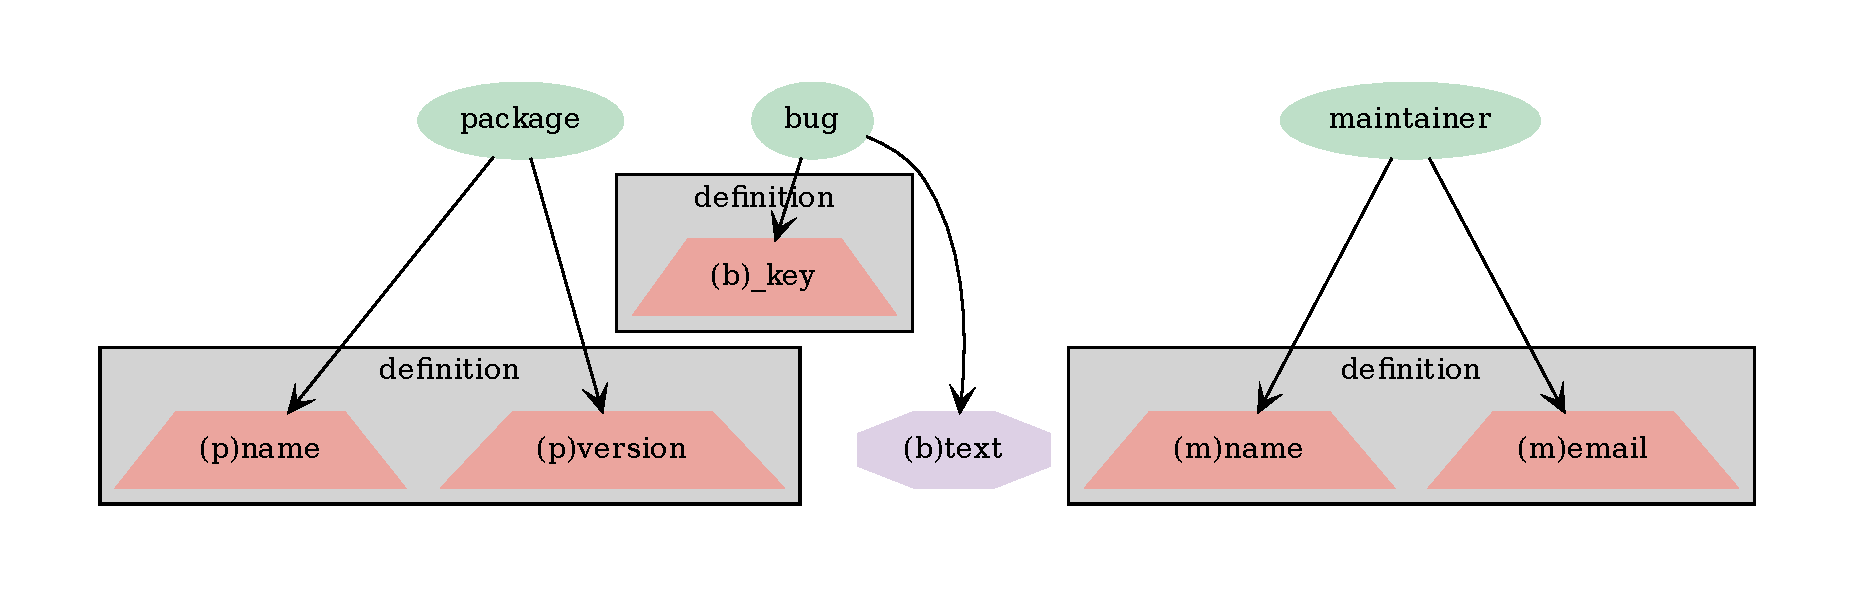
\includegraphics[width=0.8\textwidth]{../figs/debian-eco-vc2fields} &
            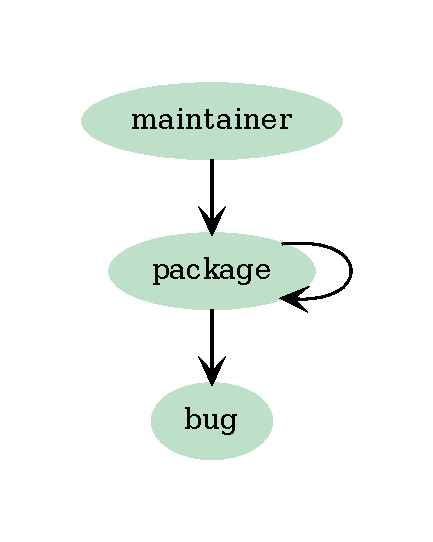
\includegraphics[width=0.2\textwidth]{../figs/debian-eco-vc2vc} \\
        \end{tabular}
        \caption{\textbf{Left}: \textbf{Right}:.}\label{fig:schema}
    \end{figure}


    Represent as a property graph.

    Use GraphCast for processing: <https://growgraph.github.io/graphcast/>.

    A framework for transforming tabular (CSV, SQL) and hierarchical data (JSON, XML) into property graphs and ingesting them into graph databases (ArangoDB, Neo4j).

    Describe relations: package, maintainer, dependencies, bugs.


    \section{Use Cases}

    Enhanced Use Cases:

    - Tracking and validating package dependencies.
    - Identifying and analyzing vulnerability propagation.
    - Assessing license compatibility and compliance.
    - Auditing build reproducibility across packages.
    - Highlighting Areas Lacking Reproducible Builds.
    - Mapping Community Needs: Linking data from platforms like "grow-your-ideas" with package metadata to identify areas lacking attention
    - Informing Funding Decisions: Providing data-driven insights to allocate resources effectively, ensuring that critical community needs are addressed.

    Community Collaboration: Understand how this approach can foster collaboration within the Debian community, providing tools for maintainers, developers, and researchers to contribute and benefit from shared insights.


    \section{Conslusion}


    Present in this repository:
    https://github.com/alexander-belikov/deb-kg

    \bibliographystyle{plain}
    \bibliography{refs}

\end{document}
